\documentclass[10pt,a4paper]{article}
\usepackage[utf8x]{inputenc}
\usepackage{amsmath}
\usepackage{amsfonts}
\usepackage{amssymb}
\usepackage{graphicx}
\usepackage{Sweave}

\newcommand{\DR}{package \texttt{DMwR}}

\author{Luis Torgo\\FCUP - LIAAD/INESC Tec\\University of Porto\\
  \texttt{ltorgo@inescporto.pt}, \texttt{ltorgo@fc.up.pt}}
\title{An Infra-Structure for\\ Experimental Comparisons of Predictive Models}

\begin{document}
%\SweaveOpts{concordance=TRUE}
  
\maketitle

\begin{abstract}
  This document describes an infra-structure available in package
  \textbf{DMwR} that facilitates carrying out experimental comparisons
  between different predictive models for different data sets using
  several different experimental methodologies to estimate their
  predictive performance.
\end{abstract}

\section{Introduction}

The goal of this document is to describe the infra-structure that is
available in \DR~\cite{Tor10} to carry out experimental comparisons
between different approaches to predictive tasks. This is a general
infra-structure in the sense that it allows the user to specify the
overall process taken to the task and then takes care of the process
of obtaining reliable estimates of its predictive performance
using  some experimental methodology. The infra-structure
implements the most frequently used experimental methodologies for
performance estimation, namely: (i) cross validation, (ii) holdout,
(iii) leave one out cross validation, (iv) bootstrap and also (v)
Monte-Carlo experiments for time series forecasting tasks.

Experimental methodologies for performance estimation are iterative
processes that repeat the modelling task several times using different
data samples with the goal of improving the accuracy of the
estimates. These estimates are the results of aggregating the scores
obtained on each of the repetitions. For each of these
repetitions different training and testing samples are generated and
the process being evaluated is "asked" to: (i) obtain the predictive
model using the training data, and then (ii) use this model to obtain
predictions for the respective test sample, which in turn (iii) can be
used to calculate the scores of the performance metrics being
estimated. This means that there is a workflow that starts with a
predictive task for which training and testing samples are given, and
that it should produce as result the scores of the performance metrics
being estimated. There are far too many possible approaches and
sub-steps for the implementation of this workflow.  To ensure full
generality of the infra-structure, we ask the user to provide a
function that implements this workflow for each of the predictive
approaches he/she wishes to compare and/or evaluate. This function can
be parametrizable in the sense that there may be variants of the
workflow that the user wishes to evaluate and/or compare. Still, the
goal of this workflow implementation functions is very clear: (i)
receive as input a predictive task for which training  and  test
samples are given, as well as any eventual workflow specific parameters; and
(ii) produce as result a set of scores for the evaluation metrics
being estimated. These scores should be obtained by applying some
modeling technique to the training sample and then use the resulting
to model to obtain predictions for the test sample. These predictions
should then be used to obtain the scores of the predictive metrics the
user is interested in obtaining reliable estimates.

The infra-structure we describe here provides means for the user to
indicate: (i) a set of predictive tasks with the respective data sets;
(ii) a set of workflows and respective variants; and (iii) an
experimental methodology. The infra-structure then takes care of all
the process of experimentally comparing the different approaches on
the different tasks, producing as result an object that can be
explored in different ways to obtain the results of the experimental
comparisons. During the experiments the infra-structure will call the
user-supplied workflow functions with different train and test
samples. 

The infra-structure also provides several utility functions
to explore the object resulting from the experiments, for instance to
obtain statistics of the results both in textual format as well as
visually. Moreover, it also provides functions that carry out
statistical significance tests based on the outcome of the
experiments. 

Finally, the infra-structure provides utility functions
implementing frequently used workflows for common modelling techniques, as
well as functions that facilitate the automatic generation of variants
of workflows by specifying sets of parameters that the user wishes to
consider in the comparisons.

\section{A Simple Illustrative Example}\label{sec:simpleEx}

Let us assume we are interested in comparing several variants of
an SVM on the
\textbf{Iris} classification problem. More specifically, we want to
obtain a reliable estimate of the error rate of these variants using
10-fold cross validation. The following code illustrates how these
estimates could be obtained with our proposed infra-structure.

\begin{Schunk}
\begin{Sinput}
> library(DMwR)
> library(e1071)
> data(iris)
> res <- experimentalComparison(
+          dataset(Species ~ .,iris),
+          variants('standardWF',
+                   learner='svm',
+                   learner.pars=list(cost=c(1,5,10),gamma=c(0.1,0.001))
+                  ),
+          cvSettings(1,10,123))
\end{Sinput}
\end{Schunk}

This simple example illustrates several key concepts of our
infra-structure. First of all, we have the main function  -
\texttt{experimentalComparison()}, which is used to carry out
the experimental comparisons. It has 3 arguments: (i) a vector of
predictive tasks (in the example a single one); (ii) a vector of workflows; and (iii) the
experimental settings. 

Predictive tasks are S4 objects of class
\textbf{dataset}. This class, also defined in our infra-structure,
describes a predictive task by: (i) a formula; (ii) the source data
set (an R data frame); and (iii) an optional name of the task (a
string). 

Workflows are S4 objects of class \textbf{learner}, which are also
defined within the infra-structure. These objects include two pieces
of information: (i) the name of the function (a string) implementing the
workflow; and (ii) the list of parameters to this function. The
function will be called from within 
\texttt{experimentalComparison()}  with a formula in the first
argument, a training sample (a data frame) on the second argument, a
test sample (another data frame) on the third, and then all the parameters
the user specifies in the list of parameters used when creating the
\textbf{learner} object. This means that the object
\texttt{learner('svmTrial',pars=list(cost=10,gamma=0.5))}, if used in a
call to \texttt{experimentalComparison}, will 
 generate calls of the type
\texttt{svmTrial(\textit{someFormula}, \textit{someTrainingSample}, \textit{someTestSample}, cost=10,
  gamma=0.5)}. In the illustrative example with \textbf{Iris} we are using the function \texttt{variants()} from our package to automatically
generate a vector of \textbf{learner} objects. This function can be used
to generate different variants of a workflow function using all
combinations of different parameters of the workflow. In the code
above the workflow function is \texttt{standardWF()} which is another
auxiliar function we provide. This function implements a typical
workflow for different modeling techniques that are indicated through
its parameter \texttt{learner}. Above we are using it to generate
variants of the \texttt{svm()} model, which is an implementation of an SVM available in package \texttt{e1071}~\cite{}.  Later we will provide
more details on the \texttt{standardWF} function. For now we can think of the call
to the \texttt{variants()} function as generating the following vector:\linebreak
\begin{verbatim}
c(learner('standardWF',
          pars=list(learner='svm',
                    learner.pars=list(cost=1,gamma=0.1))
         ), 
  learner('standardWF',
          pars=list(learner='svm',
                    learner.pars=list(cost=5,gamma=0.1))
         ),
...
...
 ) 
\end{verbatim}
 
The workflow implemented through function \texttt{standardWF()} by
default calculates the error rate of the used modeling techniques if
handling classification tasks, though we will see later that we can
specify other metrics.

Finally, the third parameter of the function
\texttt{experimentalComparison()} specifies the experimental settings
to use in the estimation process. It is an S4 object of class
\textbf{expSettings} that in effect is an union that includes among
others the S4 class \textbf{cvSettings}. Objects of this latter class
include information on the number of repetitions of the cross
validation process (in our example 1 single repetition, which is the
default), the number of folds (10 above, which is also the default),
the random number seed and a logical indicating whether stratified
samples should be used (defaulting to \texttt{FALSE}, i.e. no stratification).

The result of the call to \texttt{experimentalComparison()} is an S4
object of the class \textbf{compExp}. These objects tipically are not
 directly explored by the end-user so we ommit their
details here\footnote{Interested readers may have a look at the corresponding
  help page - \texttt{class?compExp} .}. There are several utility
functions that allow the users to explore the results of the
experimental comparisons. Here are a few illustrative examples:


\begin{Schunk}
\begin{Sinput}
> summary(res)
\end{Sinput}
\begin{Soutput}
== Summary of a  Cross Validation  Experiment ==

 1 x 10 - Fold Cross Validation run with seed =  123 

* Data sets ::  iris
* Learners  ::  svm.v1, svm.v2, svm.v3, svm.v4

* Summary of Experiment Results:


-> Datataset:  iris 

	*Learner: svm.v1 
               err
avg     0.02666667
std     0.04661373
min     0.00000000
max     0.13333333
invalid 0.00000000

	*Learner: svm.v2 
               err
avg     0.04000000
std     0.06440612
min     0.00000000
max     0.20000000
invalid 0.00000000

	*Learner: svm.v3 
              err
avg     0.5733333
std     0.1967639
min     0.3333333
max     0.8666667
invalid 0.0000000

	*Learner: svm.v4 
               err
avg     0.09333333
std     0.06440612
min     0.00000000
max     0.20000000
invalid 0.00000000
\end{Soutput}
\end{Schunk}

The generic function \texttt{summary} allows us to obtain the
estimated scores for each compared approach on each predictive
task. For each performance metric (in this case only the error rate),
the function shows the estimated average performance, the standard
error of this estimate as well as minimum and maximum scores on the
different iterations of the experimental comparison. Moreover,
information is also given on eventual failures on some of the
iterations.

The best scores for each predictive task can be obtained as follows:

\begin{Schunk}
\begin{Sinput}
> bestScores(res)
\end{Sinput}
\begin{Soutput}
$iris
    system      score
err svm.v1 0.02666667
\end{Soutput}
\end{Schunk}

The generic function \texttt{plot} can be used to obtain a graphical
display of the distribution of performance metrics across the
different iterations of the estimation process using box-plots, as
show in Figure~\ref{fig:ex1Iris}. In this case we can observe that the
performance is constant on all variants (which could also be observed
in the output of \texttt{summary}), which indicates that the different
levels of pruning are having no effect for this simple predictive
task.

\begin{figure}[ht]
  \centering
\begin{Schunk}
\begin{Sinput}
> plot(res)
\end{Sinput}
\end{Schunk}
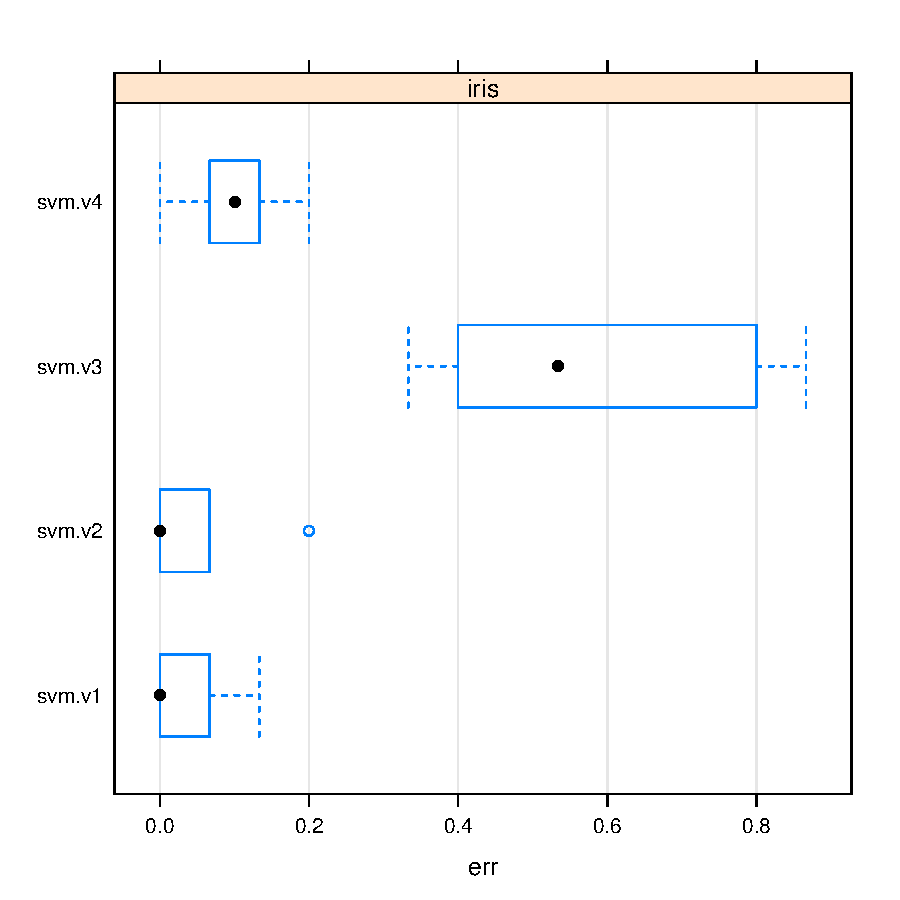
\includegraphics{compExps-005}
  \caption{The distribution of the error rate on the 10 folds.}
  \label{fig:ex1Iris}
\end{figure}

You might have observed that the infra-structure uses some IDs to
describe each variant (e.g. \texttt{svm.v1}). The user can check
the parameter configuration corresponding to some ID as follows:

\begin{Schunk}
\begin{Sinput}
> getVariant('svm.v1',res)
\end{Sinput}
\begin{Soutput}
Learner::  "standardWF" 

Parameter values
	 learner.pars  =  structure(list(cost = 1, gamma = 0.1), .Names = c("cost", "gamma" )) 
	 learner  =  "svm" 
\end{Soutput}
\end{Schunk}

\section{Predictive Tasks}

Predictive tasks are data analysis problems where we want to obtain a
model of an unknown function $Y=f(X_1, X_2, \cdots, X_p)$ that relates
a target variable $Y$ with a set of $p$ predictors $X_1, X_2, \cdots,
X_p$. The model is usually obtained using a sample of $n$ observations
of the mapping of the unknown function, $D=\{\langle \mathbf{x}_i,
Y_i\rangle\}_{i=1}^n$, where $\mathbf{x}_i$ is a vector with the $p$
predictors values.  These data sets in R are usually stored in data
frames, and formula objects are used to specify the form of the
functional dependency that we are trying to model, i.e. which is the
target variable and the predictors.

Objects of class \textbf{dataset} encapsulate the information of a
predictive task, i.e. the functional form and the data required for
solving it. For convinience they also allow the user to assign a name
to each task. These S4 objects can be created using the construtor
function \texttt{dataset()}, as seen in the following example:

\begin{Schunk}
\begin{Sinput}
> data(iris)
> dataset(Species ~ .,iris,'irisTask')
\end{Sinput}
\begin{Soutput}
Task Name ::  irisTask
Formula   :: Species ~ .
Task Data ::

'data.frame':	150 obs. of  5 variables:
 $ Species     : Factor w/ 3 levels "setosa","versicolor",..: 1 1 1 1 1 1 1 1 1 1 ...
 $ Sepal.Length: num  5.1 4.9 4.7 4.6 5 5.4 4.6 5 4.4 4.9 ...
 $ Sepal.Width : num  3.5 3 3.2 3.1 3.6 3.9 3.4 3.4 2.9 3.1 ...
 $ Petal.Length: num  1.4 1.4 1.3 1.5 1.4 1.7 1.4 1.5 1.4 1.5 ...
 $ Petal.Width : num  0.2 0.2 0.2 0.2 0.2 0.4 0.3 0.2 0.2 0.1 ...
\end{Soutput}
\end{Schunk}

We should remark that the objects of this class only store the data
required for the specified task, as it should be clear from this other
simple example:

\begin{Schunk}
\begin{Sinput}
> data(iris)
> dataset(Species ~ Petal.Length + Sepal.Length,iris,'ShortIrisTask')
\end{Sinput}
\begin{Soutput}
Task Name ::  ShortIrisTask
Formula   :: Species ~ Petal.Length + Sepal.Length
Task Data ::

'data.frame':	150 obs. of  3 variables:
 $ Species     : Factor w/ 3 levels "setosa","versicolor",..: 1 1 1 1 1 1 1 1 1 1 ...
 $ Petal.Length: num  1.4 1.4 1.3 1.5 1.4 1.7 1.4 1.5 1.4 1.5 ...
 $ Sepal.Length: num  5.1 4.9 4.7 4.6 5 5.4 4.6 5 4.4 4.9 ...
\end{Soutput}
\end{Schunk}

So, although we have supplied the full data frame to the constructor
function, as the task only uses 3 of the columns, the resulting
\textbf{dataset} object only includes the information on the columns
required for this task.

\section{Workflows}

Experimental methodologies work most of the times by re-sampling the
available data set $D$ in order to create different train and test
samples from $D$. The goal is to estimate the predictive performance
of a proposed workflow to solve the task, by using these different
samples to increase our confidence on the estimates. This workflow
consists on the process of obtaining a model from a given training
sample and then use it to obtain predictions for the given test
set. This process can include several steps, e.g. specific data
pre-processing steps, and may use any modeling approach, eventually
being proposed by the user. 

\subsection{User-defined Workflows}

With the goal of ensuring that the
proposed infra-structure is able to cope with all these possible usage
scenarios, we ask the user to take care of the writing of a function
implementing each workflow being compared/evaluated. These
user-defined workflow functions should be written assuming that the
first three arguments are: (i) the formula defining the predictive
task; (ii) the provided training sample; and (iii) the test sample
where to evaluate the obtained model. The functions may eventually
accept other arguments with specific parameters of the workflow. The
following is a general sketch of a user-defined workflow function:

\begin{Verbatim}
myWorkFlow <- function(form,train,test,...) {
  require(mySpecialPackage,quietly=T)
  myTrain <- mySpecificPreProcessingSteps(train)
  myModel <- myModelingTechnique(form,myTrain,...)
  preds <- predict(myModel,test)
  scores <- mySpecialEvaluationMetrics(resp(form,test),preds)
  scores
}
\end{Verbatim}

Not all workflows will require all these steps, though some may even
require more. This is clearly something that is up to the user. The
only requirements for these functions are: (i) the first 3 arguments
of the workflow function should be the formula, train and test data
frames; and (ii) the result of the function should be \textbf{a named
  vector with the values of the metrics} being estimated. The names of
the positions of this vector will typically be the names of the
corresponding metrics.

The sketch shown above also illustrates the use of the function
\texttt{resp()} that can be used to obtain the values of the target
variable given a formula and a data frame.

Users should write one such workflow function for each process they
want to evaluate/compare. As mentioned before these functions may
accept further parameters on top of the 3 mandatory parameters. These
extra parameters will typically be parameters of the modeling
technique being used in the workflow but it is up to the user to
control this. As we have seen in Section~\ref{sec:simpleEx} we provide
the function \texttt{variants()} to facilitate the specification of
different variants of any workflow function by trying all combinations
of several of its specific parameters. For instance, if the modeling
function in the above example workflow (function
\texttt{myModelingTechnique()}) had an integer parameter \texttt{x}
and a Boolean parameter \texttt{y}, we could generate several
\textbf{learner} objects to be evaluated/compared using the
\texttt{experimentalComparison()} function, as follows:

\begin{Schunk}
\begin{Sinput}
> variants('myWorkFlow',x=c(0,3,5,7),y=c(T,F))
\end{Sinput}
\end{Schunk}

This would generate 8 variants of the same workflow with all
combinations of the specified values for the 2 parameters.  This means
that any parameter of the \texttt{variants()} function that has more
than one element is assumed to be a source for generation of
variants. There may be situations where this is not desirable, because
a particular argument of the workflow function is supposed to be a
vector. In these cases the user needs to ``tell'' the
\texttt{variants()} function that it should not generate variants from
the values of that parameter. Suppose that on the above example the
parameter \texttt{x} takes as values a vector, and thus your meaning
in the above statment is that you only have two variants of the
workflow (the different values of the other parameter). You could get
that results by calling the \texttt{variants()} function as follows:

\begin{Schunk}
\begin{Sinput}
> variants('myWorkFlow',x=c(0,3,5,7),y=c(T,F),as.is=c('x'))
\end{Sinput}
\end{Schunk}

While the previous call would generate 8 variants, this one only generates 2.

Let us see a concrete example of a user supplied workflow
function. Imagine we want to evaluate a kind of ensemble model formed
by a regression tree and a multiple linear regression model on an
algae blooms data set~\cite{Tor10}. Moreover, let us suppose we are
interested in using the correlation between the predictions and true
values as evaluation metric. We could start by writting the following
workflow function that implements our modeling approach:

\begin{Schunk}
\begin{Sinput}
> RLensemble <- function(f,tr,ts,weightRT=0.5,step=F,...) {
+   require(DMwR,quietly=F)
+   noNAsTR <- knnImputation(tr)
+   noNAsTS <- knnImputation(ts)
+   r <- rpartXse(f,tr,...)
+   l <- lm(f,noNAsTR)
+   if (step) l <- step(l,trace=0)
+   pr <- predict(r,ts)
+   pl <- predict(l,noNAsTS)
+   ps <- weightRT*pr+(1-weightRT)*pl
+   c(correlation=cor(resp(f,ts),ps))
+ }
\end{Sinput}
\end{Schunk}

This workflow starts by building two modified samples of the training
and testing sets, with the \texttt{NA} values being filled in using a
nearest neighbour strategy (see the help page of the function
\texttt{knnImputation()} of package \textbf{DMwR} for more
details). These versions are to be used by the \texttt{lm()} function
that is unable to cope with cases with missing values. After obtaining
the two models and their predictions the function calculates a
weighted average of both predictions before obtaining and returning
the respective correlation score.

To evaluate different variants of this workflow we could run the
following experiment:

\begin{Schunk}
\begin{Sinput}
> data(algae)
> expRes <- experimentalComparison(
+   dataset(a1 ~ .,algae[,1:12],'alga1'),
+   variants('RLensemble',
+            se=c(0,1),step=c(T,F),weightRT=c(0.4,0.5,0.6)),
+   bootSettings(1234,100))
\end{Sinput}
\end{Schunk}

In this experimental comparison we have used 100 repetitions of a
bootstrap estimation procedure as experimental methodology (further
details on this and other methodologies will be given later), to
compare 12 variants of our workflow. 

\subsection{Generic Workflows}

Writing workflow functions may be tedious on large comparisons,
particularly when few details change among them. Moreover, the most
frequent use of our infra-structure will probably be to compare
existing modeling techniques on one or more problems. This means that
the most frequently used workflows will essentially build a model
using some existing algorithm, obtain its predictions and then
calculate some standard prediction error metric. In this context, we
have provided a generic workflow function that carries out this type
of process for any modeling technique. The idea is to save the user
from having to write these functions provided his/her workflow fits
this generic schema.

\subsubsection{Classification and Regression Tasks}

Function \texttt{standardWF()} implements a typical workflow for both
classification and regression tasks. Apart from a formula, a training set data frame and a test set data frame, this function has the following parameters that help the user to specify is intended workflow:

\begin{description}
\item[learner] - the name of a R function that obtains a model from the training data. This function will be called with a formula in the first argument and the training set data frame in the second.
\item[learner.pars] - a list specifying any extra parameter settings that should be added to the formula and training set, at the time the learner function is called (defaults to \texttt{NULL}).
\item[predictor] - the name of a R function that is able to obtain the predictions of the model obtained with \texttt{learner}. This function will be called with the object resulting from the \texttt{learner} call on the first argument and the test set data frame in the second (it defaults to function ``predict'').
\item[predictor.pars] - a list specifying any extra parameter settings that should be added to the model and test set, at the time the predictor function is called (defaults to \texttt{NULL}).
\item[evaluator] - the name of a R function that is able to calculate the evaluation metrics you want to estimate based on the predictions of the model and the true values of the target variable on the given test set (it will default to \texttt{class.eval()} function if it is a classification task, and to \texttt{regr.eval()} if a regression task - check the respective help pages to see what are the default metrics that are calculated for each). This function will be called with the values of the target variable in the test set on the first argument and with the result of the call to the predictor function on the second.
\item[evaluator.pars] -  a list specifying any extra parameter settings that should be added to the true values and predictions, at the time the evaluator function is called (defaults to \texttt{NULL}). A typical usage here would be to use the parameter \texttt{stats} of functions \texttt{class.eval()} and \texttt{regr.eval()} to specify the metrics you want to calculate, provided you are using these functions as evaluators.
\end{description}


Below you find an example of one of the most frequent type of
comparisons users carry out - checking which is the ``best'' model for
a given predictive task. Let us restrict the search to a small set of
models for illustrative purposes and let us play with the well-known
Boston housing regression task:

\begin{Schunk}
\begin{Sinput}
> data(Boston,package='MASS')
> library(e1071)
> library(randomForest)
> bostonRes <- experimentalComparison(
+   dataset(medv ~ .,Boston),
+   variants('standardWF',learner=c('rpartXse','svm','randomForest')),
+   cvSettings(1,10)
+   )
\end{Sinput}
\end{Schunk}

Notice that on this simple example we have used all modeling tools
with their default parameter settings which is not necessarly a good
idea when we are looking for the best performance. Still, the goal of
this illustration is to show you how simple this type of experiments
can be if you are using a standard workflow setting. In case you want
to use the modeling tools with other parameter settings then you
should separate them in different \texttt{variants()} calls, as shown
in the following example:

\begin{Schunk}
\begin{Sinput}
> data(Boston,pacakge='MASS')
> library(e1071)
> library(randomForest)
> bostonRes <- experimentalComparison(
+   dataset(medv ~ .,Boston),
+   c(variants('standardWF',
+              learner='rpartXse',
+              learner.pars=list(se=c(0,1))
+             ),
+     variants('standardWF',
+              learner='svm',
+              learner.pars=list(cost=c(1,3,5),gamma=c(0.01,0.1))
+             ),
+     variants('standardWF',
+              learner='randomForest',
+              learner.pars=list(ntree=c(500,1000))
+             )
+     ),
+   cvSettings(1,10)
+   )
\end{Sinput}
\end{Schunk}

Notice that this code will involve evaluating 10 models through
10-fold cross validation. 


\subsubsection{Time Series Tasks}

Our infra-structure also includes another generic workflow function
that is specific for predictive tasks with time-dependent data
(e.g. time series forecasting problems). This workflow function
implements two different approaches to the problem of training a
forecasting model with a set of time-dependent data and then use it to
obtain predictions for a test set in the future. These two approaches
contrast with the standard approach of learning a model with the
available training sample and then use it to obtain predictions for
all test period. This standard approach could be used with the already
described \texttt{standardWF()} function. However, there are
alternatives to this procedure, two of the most common being the
sliding and growing window approaches, which are implemented in our
provided workflow function for time series.

Predictive tasks for time-dependent data are different from standard
classification and regression tasks because they require that the test
samples have time stamps that are more recent then training
samples. In this context, experimental methodologies handling these
tasks typically do not shuffle the observations to avoid these
effects. The most common setup is that we have a $L$ time steps
training window containing samples in the period $[t_1,t_L]$ and a $F$
time steps test window typically containing the observations in the
time window $[t_{L+1},t_{L+F}]$. In this context, the idea of the
sliding window method is that if we want a prediction for time point
$t_k$ belonging to the test interval $[t_{L+1},t_{L+F}]$ then we can
assume that all data from $t_{L+1}$ till $t_{k-1}$ is already past,
and thus usable by the model. In this context, it may be wise to use
this new data in the interval $[t_{L+1},t_{k-1}]$ to update the
original model obtained using only the training period data. This is
particularly advisable if we suspect that the conditions may have
changed since the training period has ended. Model updating using the
sliding window method is carried out by using the data in the $L$ last
time steps, i.e. every new model is always obtained using the last $L$
data observations, as if the training window was slided forward in
time. Our \texttt{timeseriesWF()} function implements this idea for
both time series with a numeric target variable and a nominal target
variable. This function has a parameter (\texttt{type}) that if set to
``slide'' will use a sliding window approach. As with the
\texttt{standardWF()} function, this \texttt{timseriesWF()} function
also accepts parmeters specifying the learner, predictor, evaluator
and their respective parameters. Moreover, this function also includes
an extra parameter, named \texttt{relearn.step}, which allows the user
to establish the frequency of model updating. By default this is every
new test sample, i.e. $1$, but the user may set a less frequent
model-updating policy by using higher values of this parameter.  The
idea of the growing window method is very similar. The only difference
is on the data used when updating the models. Whilst sliding window
uses the data occurring in the last $L$ time steps, growing window
keeps increasing the original training window with the newly available
data points, i.e. the models are obtained with increasing size
training samples. By setting the parameter \texttt{type} to ``grow''
you get the \texttt{timseriesWF()} function to use this method.


\section{Estimation Methodologies}\label{sec:expMeth}

There are different ways of providing reliable estimates of the
predictive performance of a model. Our infra-structure implements some
of the most common estimation methods. In this section we
briefly describe them and provide short illustrative examples of their
use.

\subsection{Cross Validation}

$k$-Fold cross validation (CV) is one of the most common 
methods to estimate the predictive performance of a model. By
including an S4 object of class \textbf{cvSettings} in the third
argument of function \texttt{experimentalComparison()} we can carry
out experiments of this type.

Function \texttt{cvSettings()} can be used as a constructor of objects
of class \textbf{cvSettings}. It accepts the following arguments:

\begin{description}
\item[cvReps] - the number of repetitions of the $k$-fold CV experiment (default is $1$)
\item[cvFolds] - the number of $k$ folds to use (default is $10$)
\item[cvSeed] - the random number generator seed to use (default is $1234$)
\item[strat] - whether to use stratified samples (default is \texttt{FALSE})
\item[dataSplits] - a data frame containing user-supplied data splits
  for each of the folds and repetitions (check the help page of the
  class for further details). This parameter defaults to
  \texttt{NULL}, i.e. no user-supplied splits, they are decided
  internally by the infra-structure.
\end{description}

Bellow you can find a small illustration using the Breast Cancer data
set available in package \textbf{mlbench}. On this example we compare
some variants of an SVM using a $3\times 10-$fold cross validation
process with stratified sampling because one of the two classes has a
considerably lower frequency.

\begin{Schunk}
\begin{Sinput}
> data(BreastCancer,package='mlbench')
> library(e1071)
> bc <- knnImputation(BreastCancer[,-1])
> bcExp <- experimentalComparison(
+   dataset(Class ~ .,bc,'BreastCancer'),
+   variants('standardWF',
+            learner='svm',
+            learner.pars=list(cost=c(1,5),gamma=c(0.01,0.1))
+           ),
+   cvSettings(3,10,1234,T))
\end{Sinput}
\end{Schunk}

\subsection{Bootstrapping}

Bootstrapping or boostrap resampling is another well-known
experimental methodology that is implemented in our
infra-structure. By including an S4 object of class
\textbf{bootSettings} in the third argument of function
\texttt{experimentalComparison()} we can carry out experiments of this
type.

Function \texttt{bootSettings()} can be used as a constructor of
objects of class \textbf{bootSettings}. It accepts the following
arguments:

\begin{description}
\item[bootSeed] - the random number generator seed to use (default is $1234$)
\item[bootReps] - the number of repetitions of the bootstrap experiment (default is $50$)
\item[dataSplits] - a data frame containing user-supplied data splits
  for each of the repetitions (check the help page of the
  class for further details). This parameter defaults to
  \texttt{NULL}, i.e. no user-supplied splits, they are decided
  internally by the infra-structure.
\end{description}

Bellow you can find a small illustration using the Servo data set available in package \textbf{mlbench}. On this example we compare some variants of an artificial neural network using 200 repetitions of a boostrap experiment.

\begin{Schunk}
\begin{Sinput}
> data(Servo,package='mlbench')
> library(nnet)
> nnExp <- experimentalComparison(
+   dataset(Class ~ .,Servo),
+   variants('standardWF',
+            learner='nnet',
+            learner.pars=list(trace=F,linout=T,size=c(3,5),decay=c(0.01,0.1))
+           ),
+   bootSettings(1234,200))
\end{Sinput}
\end{Schunk}

\subsection{Holdout}

The Holdout is another frequently used experimental methodology,
particularly for large data sets. To carry out this type of
experiments in our infra-structure we can include an S4 object of
class \textbf{hldSettings} in the third argument of function
\texttt{experimentalComparison()}.

Function \texttt{hldSettings()} can be used as a constructor of
objects of class \textbf{hldSettings}. It accepts the following
arguments:

\begin{description}
\item[hldReps] - the number of repetitions of the Holdout experiment (default is $1$)
\item[hldSz] - the percentage  of cases (a number between 0 and 1) to leave as holdout (test set) (default is $0.3$)
\item[hldSeed] - the random number generator seed to use (default is $1234$)
\item[strat] - whether to use stratified samples (default is \texttt{FALSE})
\item[dataSplits] - a data frame containing user-supplied data splits
  for each of the repetitions (check the help page of the
  class for further details). This parameter defaults to
  \texttt{NULL}, i.e. no user-supplied splits, they are decided
  internally by the infra-structure.
\end{description}

Notice that when we have a number of repetitions larger than one what
we have is actually usually known as random subsampling.

The following is a small illustrative example of the use of the
Holdout with the LetterRecognition classification task from package
\textbf{mlbench}.

\begin{Schunk}
\begin{Sinput}
> data(LetterRecognition,package='mlbench')
> ltrExp <- experimentalComparison(
+   dataset(lettr ~ .,LetterRecognition),
+   variants('standardWF',
+            learner='rpartXse',
+            learner.pars=list(se=c(0,1)),
+            predictor.pars=list(type='class')
+            ),
+   hldSettings(3,0.3))
\end{Sinput}
\end{Schunk}

\subsection{Leave One Out Cross Validation}

Leave one out cross validation is a type of cross validation method
that is mostly used for small data sets. You can think of leave one
out cross validation as a $k$-fold cross validation with $k$ equal to
the size of the available data set. To carry out this type of
experiments in our infra-structure we can include an S4 object of
class \textbf{loocvSettings} in the third argument of function
\texttt{experimentalComparison()}.

Function \texttt{loocvSettings()} can be used as a constructor of
objects of class \textbf{loocvSettings}. It accepts the following
arguments:

\begin{description}
\item[loocvSeed] - the random number generator seed to use (default is $1234$)
\item[verbose] - whether the execution of the experiments should provide a verbose form of output (default is \texttt{FALSE})
\end{description}


The following is a small illustrative example of the use of the
Holdout with the LetterRecognition classification task from package
\textbf{mlbench}.

\begin{Schunk}
\begin{Sinput}
> data(iris)
> library(e1071)
> irisExp <- experimentalComparison(
+   dataset(Species ~ .,iris),
+   variants('standardWF',
+            learner='svm',
+            learner.pars=list(cost=c(1,10))
+            ),
+   loocvSettings())
\end{Sinput}
\end{Schunk}
\subsection{Monte Carlo Experiments}

Monte Carlo experiments are similar to random subsampling (or repeated
Holdout) in the sense that they consist of repeating a learning +
testing cycle several times using different data samples. The main
different lies on the way the samples are obtained. In Monte Carlo
experiments the original order of the observations is respected and
train and test splits are obtained such that the testing samples
appear ``after'' the training samples, thus being the methodology of
choice when you are comparing time series forecasting models. The idea
of Monte Carlo experiments is the following: (i) given a data set
spanning from time $t_1$ till time $t_N$, (ii) given a training set
time interval size $L$ and a test set time interval size $F$, such
that $T+F < N$, (iii) Monte Carlo experiments generate $R$ random time
points from the interval $[t_{1+T},t_{N-F}]$, and then (iv) for each
of these $R$ time points they generate a training set with data in the
interval $[t_{R-T+1},t_{R}]$ and a test set with data in the interval
$[t_{R+1},t_{R+F}]$. Using this process $R$ train+test cycles are
carried out using the user-supplied workflow function, and the
experiment estimates result from the average of the $R$ scores as
usual.

To carry out this type of experiments in our infra-structure we can
include an S4 object of class \textbf{mcSettings} in the third
argument of function \texttt{experimentalComparison()}.

The function \texttt{mcSettings()} can be used as a constructor of
objects of class \textbf{mcSettings}. It accepts the following
arguments:

\begin{description}
\item[mcReps] - the number of repetitions of the Monte Carlo experiment (default is $10$)
\item[mcTrain] - the percentage (a number between 0 and 1) or the actual number of cases to use in the training samples (default is $0.25$)
\item[mcTest] - the percentage (a number between 0 and 1) or the actual  number of cases to use in the test samples (default is $0.25$)
\item[mcSeed] - the random number generator seed to use (default is $1234$)
\item[dataSplits] - a data frame containing user-supplied data splits
  for each of the repetitions (check the help page of the
  class for further details). This parameter defaults to
  \texttt{NULL}, i.e. no user-supplied splits, they are decided
  internally by the infra-structure.
\end{description}

The following is a small illustrative example using the quotes of the
SP500 index. This example compares two random forests with 500
regression trees, one applying in a standard way, and the other using
a sliding window with a relearn step of every 5 days. The experiment
uses 10 repetitions of a train+test cycle using 50\% of the available
data for training and 25\% for testing.

\begin{Schunk}
\begin{Sinput}
> library(quantmod)
> library(randomForest)
> getSymbols('^GSPC',from='2008-01-01',to='2012-12-31')
> data.model <- specifyModel(
+   Next(100*Delt(Ad(GSPC))) ~ Delt(Ad(GSPC),k=1:10)+Delt(Vo(GSPC),k=1:3))
> data <- modelData(data.model)
> colnames(data)[1] <- 'PercVarClose'
> spExp <- experimentalComparison(
+   dataset(PercVarClose ~ .,data,'SP500_2012'),
+   c(standRF=learner('standardWF',
+                     pars=list(learner='randomForest',
+                               learner.pars=list(ntree=500))
+                    ),
+     slideRF=learner('timeseriesWF',
+                     pars=list(learner='randomForest',
+                               learner.pars=list(ntree=500,relearn.step=5))
+                    )
+     ),
+   mcSettings(10,0.5,0.25))
\end{Sinput}
\end{Schunk}



\section{Statistical Significance of Differences}

The experimental methodologies that we have presented in the previous
section allow the user to obtain estimates of the predictive
performance of different workflows or variants of these workflows, on
different predictive tasks. We have seen that by applying the
\texttt{summary} method to the objects resulting from the experiments
we can obtain the average performance for each candidate workflow on
each task. These numbers are estimates of the expected average
performance of the workflows on the respective tasks. Being estimates,
the obvious next question is to check whether the observed differences
in performance between the workflows are statistically
significant. That is the goal of the function
\texttt{compAnalysis()}. This function provides a series of pairwise
comparisons between different workflows for each predictive task, with
the goal of calculating and presenting the statistical significance of
the differences, if any.

Our experimental infra-structure ensures that all compared workflows
are run on exactly the same train+test samples on all repetitions and
for all predictive tasks. In this context, we can focus on pairwise
statistical significance tests. Given that we cannot ensure that the
different iterations are statistically independent (for instance there
may be some overlap between the training samples), we use the Wilcoxon
signed rank test to assess the statistical significance of the
differences between every pair of compared workflows. Let us see a
concrete example:


\begin{Schunk}
\begin{Sinput}
> data(LetterRecognition,package='mlbench')
> ltrExp <- experimentalComparison(
+   dataset(lettr ~ .,LetterRecognition),
+   variants('standardWF',
+            learner='rpartXse',
+            learner.pars=list(se=c(0,1)),
+            predictor.pars=list(type='class')
+            ),
+   hldSettings(3,0.3))
\end{Sinput}
\end{Schunk}

Using the \texttt{bestScores()} function we can find out the best
scoring variant of this comparison of rpartXse-based workflows,

\begin{Schunk}
\begin{Sinput}
> bestScores(ltrExp)
\end{Sinput}
\begin{Soutput}
$LetterRecognition
         system     score
err rpartXse.v1 0.1424444
\end{Soutput}
\end{Schunk}

Now we can proceed to check whether the advantage of this variant over
the others is statistically significant,

\begin{Schunk}
\begin{Sinput}
> compAnalysis(ltrExp,'rpartXse.v1')
\end{Sinput}
\begin{Soutput}
== Statistical Significance Analysis of Comparison Results ==

Baseline Learner::	 rpartXse.v1  (Learn.1)

** Evaluation Metric::	 err 

- Dataset: LetterRecognition 
        Learn.1    Learn.2 sig.2
AVG 0.142444444 0.15277778      
STD 0.005618257 0.01410903      

Legends:
Learners -> Learn.1 = rpartXse.v1 ; Learn.2 = rpartXse.v2 ; 
Signif. Codes -> 0 '++' or '--' 0.001 '+' or '-' 0.05 ' ' 1
\end{Soutput}
\end{Schunk}

The function \texttt{compAnalysis()} receives as first argument the
object resulting from the comparative experiments. The second argument
is the baseline workflow against which you want to compare the others
to. In the output this baseline will be named ``Learn.1'', and its
scores will be on the first column. After this first column we have
the scores of the other workflows (in this example only another one),
presenting also the estimated average performance and respective
standard error. In front there may be zero, one or two symbols (either
``+'' or ``-''). If no symbol is presented it means that the observed
difference is not statistically significant at the 0.05 confidence
level (i.e. with 95\% confidence). If one symbol appears it means that
the p-level is between 0.05 and 0.01, while two symbols represent
confidence higher than 99\% on the observed difference. The meaning of
the plus or minus depends on the semantics of the scores of the
evaluation metric being compared. If the lower the scores the better,
than a workflow with minus signals is significantly better than the
baseline on the first column. If the higher the metric scores the
better, than a workflow with minus signals is significantly worse than
the baseline. The interpretation of the plus signals is the inverse of
this. In the above example we observe that although
\texttt{rpartXse.v1} has a lower estimated error rate, its advantage
over \texttt{rpartXse.v2} is not statistically significant.


\section{Larger Examples}

The main advantage of the infra-structure we are proposing is to
automate large scale experimental comparisons. It is on these very
large setups that the use of the infra-structure spares more time to
the user. However, in these context the objects resulting from the
experiments are very large and some of the tools we have shown before
for exploring the results may produce over-cluttered output. In
effect, if you have an experiment involving dozens of predictive tasks
and eventually hundreds of workflow variants being compared on several
evaluation metrics, doing a plot of the resulting object is simply not
possible as the graph will be unreadable. This section illustrates
some of these cases and presents some solutions to overcome the
difficulties they bring.

Extremely large experiments may take days or weeks to complete,
depending on the available hardware. In this context, it may not be
wise to run the experiments on a single call to the
\texttt{experimentalComparison} function because if something goes
wrong in the middle you may loose lots of work. Using the random
number generation seeds that are available in all experimental
settings objects we can split the experiments in several calls and
still ensure that the same data folds are used in all
comparisons. Moreover, we will see that when all experiments are
finished we will be able to merge the objects of each call into a
single object as if we had issued a single call. Let us see an
example.

\begin{Schunk}
\begin{Sinput}
> library(DMwR)
> library(e1071)
> library(randomForest)
> library(earth)
> data(algae)
> DSs <- sapply(names(algae)[12:18],
+          function(x,names.attrs) { 
+            f <- as.formula(paste(x,"~ ."))
+            dataset(f,algae[,c(names.attrs,x)],x) 
+          },
+          names(algae)[1:11])
> WFs <- list()
> WFs$svm <- list(learner.pars=list(cost=c(10,150,300),gamma=c(0.01,0.001)))
> WFs$randomForest <- list(learner.pars=list(mtry=c(5,7),ntree=c(500,750,1500)))
> WFs$earth <- list(learner.pars=list(nk=c(10,17),degree=c(1,2),thresh=c(0.01,0.001)))
> for(d in seq_along(DSs)) {
+   for(w in names(WFs)) {
+     resObj <- paste(names(DSs)[d],w,'Res',sep='')
+     assign(resObj,
+            experimentalComparison(
+                   DSs[d],         
+                   c(
+                     do.call('variants',
+                             c(list('standardWF',learner=w),WFs[[w]]))
+                     ),
+                    cvSettings(3,10,1234))
+            )
+ 
+     save(list=resObj,file=paste(names(DSs)[d],w,'Rdata',sep='.'))
+   }
+ }
\end{Sinput}
\end{Schunk}

The above code compares 6 SVM variants with 6 random forest variants
and 8 MARS variants, on 7 algae blooms regression tasks, using
$3\times 10-$fold cross validation. Although this is not a very large
experimental comparison it still includes applying 20 different
workflow variants on 7 different prediction tasks, 30 times, i.e. 4200
train+test cycles. Instead of running all these experiments in a
single call to the function \texttt{experimentalComparison} (which
would obviously still be possible), we have made different calls for
each workflow type (SVM, random forest and MARS) and for each
predictive task. This means that each call will run all variants of a
certain workflow on a certain predictive task. The result of each of
these calls will be assigned to an object with a name composed of the
task and workflow learner. In the end each of these objects is saved
on a file with a similar name, for future loading and results
analysis. For instance, in the end there will be a file with name
``a1.svm.Rdata'' which contains an object of class \textbf{compExps}
named \texttt{a1svmRes}. This object contains the MAE and MSE
estimated scores of the SVM variants on the task of predicting the
target variable ``a1'' (one of the eight algae in this data set).

Later on, after the above experiment have completed you can load them
into R and moreover, join them into a single object, as shown below:

\begin{Schunk}
\begin{Sinput}
> nD <- paste('a',1:7,sep='')
> nL <- c('svm','randomForest','earth')
> res <- NULL
> for(d in nD) {
+   resD <- NULL
+   for(l in nL) {
+     load(paste(d,l,'Rdata',sep='.'))
+     x <- get(paste(d,l,'Res',sep=''))
+     resD <- if (is.null(resD)) x else join(resD,x,by='variants')
+   }
+   res <- if (is.null(res)) resD else join(res,resD,by='datasets')
+ }
> save(res,file='allResultsAlgae.Rdata')
\end{Sinput}
\end{Schunk}

The \texttt{join()} generic function when applied to objects of class
\textbf{compExp} allows merging of these objects across different
dimensions. Namely, such objects have the individual scores of all
experiments spread across 4 dimensions: the iterations, the
statistics, the workflows and the datasets (in effect, internally
these scores are stored as a 4-dimensions array). The argument
\texttt{by} of the \texttt{join()} function allows you to specify how
to merge the given objects. The most common situations are: (i)
merging the results of different workflows over the same data sets -
you should use ``\texttt{by='variants'}'', or (ii) merging the results
of the same workflows across different datasets - you should use
``\texttt{by='datasets'}''.

The following code can be used to check that the merging was OK, and
also to illustrate a few other utility functions whose purpose should
be obvious:


\begin{Schunk}
\begin{Sinput}
> res
\end{Sinput}
\begin{Soutput}
==  Cross Validation  Experiment ==

 3 x 10 - Fold Cross Validation run with seed =  1234 
20  learning systems
tested on  7  data sets
\end{Soutput}
\begin{Sinput}
> dsNames(res)
\end{Sinput}
\begin{Soutput}
  a1   a2   a3   a4   a5   a6   a7 
"a1" "a2" "a3" "a4" "a5" "a6" "a7" 
\end{Soutput}
\begin{Sinput}
> learnerNames(res)
\end{Sinput}
\begin{Soutput}
 [1] "regrWF.svm.v1"          "regrWF.svm.v2"          "regrWF.svm.v3"         
 [4] "regrWF.svm.v4"          "regrWF.svm.v5"          "regrWF.svm.v6"         
 [7] "regrWF.randomForest.v1" "regrWF.randomForest.v2" "regrWF.randomForest.v3"
[10] "regrWF.randomForest.v4" "regrWF.randomForest.v5" "regrWF.randomForest.v6"
[13] "regrWF.earth.v1"        "regrWF.earth.v2"        "regrWF.earth.v3"       
[16] "regrWF.earth.v4"        "regrWF.earth.v5"        "regrWF.earth.v6"       
[19] "regrWF.earth.v7"        "regrWF.earth.v8"       
\end{Soutput}
\begin{Sinput}
> statNames(res)
\end{Sinput}
\begin{Soutput}
[1] "mae" "mse"
\end{Soutput}
\end{Schunk}

With such large objects the most we can do is obtaining the best
scores or rankings of the workflows:

\begin{Schunk}
\begin{Sinput}
> bestScores(res)
\end{Sinput}
\begin{Soutput}
$a1
                    system     score
mae regrWF.randomForest.v1  10.29005
mse regrWF.randomForest.v5 233.37908

$a2
                    system      score
mae          regrWF.svm.v1   6.088107
mse regrWF.randomForest.v5 102.504805

$a3
             system     score
mae   regrWF.svm.v4  4.135187
mse regrWF.earth.v1 46.993918

$a4
                    system     score
mae          regrWF.svm.v4  1.726276
mse regrWF.randomForest.v1 13.700926

$a5
                    system     score
mae          regrWF.svm.v4  4.251671
mse regrWF.randomForest.v5 46.664527

$a6
           system      score
mae regrWF.svm.v6   5.912782
mse regrWF.svm.v6 115.938396

$a7
             system    score
mae   regrWF.svm.v4  2.50103
mse regrWF.earth.v1 26.74473
\end{Soutput}
\end{Schunk}

\begin{Schunk}
\begin{Sinput}
> rankSystems(res)
\end{Sinput}
\begin{Soutput}
$a1
$a1$mae
                  system    score
1 regrWF.randomForest.v1 10.29005
2 regrWF.randomForest.v5 10.30520
3 regrWF.randomForest.v2 10.33958
4 regrWF.randomForest.v3 10.34220
5 regrWF.randomForest.v6 10.37149

$a1$mse
                  system    score
1 regrWF.randomForest.v5 233.3791
2 regrWF.randomForest.v1 233.6848
3 regrWF.randomForest.v3 234.9995
4 regrWF.randomForest.v2 236.4458
5 regrWF.randomForest.v4 238.0586


$a2
$a2$mae
                  system    score
1          regrWF.svm.v1 6.088107
2          regrWF.svm.v4 6.225823
3          regrWF.svm.v5 6.247941
4          regrWF.svm.v6 6.261020
5 regrWF.randomForest.v5 6.803680

$a2$mse
                  system    score
1 regrWF.randomForest.v5 102.5048
2 regrWF.randomForest.v1 103.4508
3 regrWF.randomForest.v3 103.7538
4 regrWF.randomForest.v6 104.1717
5 regrWF.randomForest.v2 104.7752


$a3
$a3$mae
         system    score
1 regrWF.svm.v4 4.135187
2 regrWF.svm.v1 4.247689
3 regrWF.svm.v5 4.268914
4 regrWF.svm.v6 4.335368
5 regrWF.svm.v2 4.501554

$a3$mse
                  system    score
1        regrWF.earth.v1 46.99392
2        regrWF.earth.v5 46.99392
3        regrWF.earth.v2 47.45440
4        regrWF.earth.v6 47.48074
5 regrWF.randomForest.v5 48.30861


$a4
$a4$mae
                  system    score
1          regrWF.svm.v4 1.726276
2 regrWF.randomForest.v3 1.782650
3 regrWF.randomForest.v1 1.787691
4 regrWF.randomForest.v5 1.789502
5 regrWF.randomForest.v4 1.793457

$a4$mse
                  system    score
1 regrWF.randomForest.v1 13.70093
2 regrWF.randomForest.v3 13.84821
3 regrWF.randomForest.v5 13.86660
4 regrWF.randomForest.v4 13.99223
5 regrWF.randomForest.v6 14.04755


$a5
$a5$mae
                  system    score
1          regrWF.svm.v4 4.251671
2          regrWF.svm.v1 4.291560
3          regrWF.svm.v5 4.389319
4          regrWF.svm.v6 4.390436
5 regrWF.randomForest.v5 4.798468

$a5$mse
                  system    score
1 regrWF.randomForest.v5 46.66453
2 regrWF.randomForest.v3 46.72200
3 regrWF.randomForest.v1 46.88803
4 regrWF.randomForest.v6 47.79440
5 regrWF.randomForest.v4 47.88862


$a6
$a6$mae
         system    score
1 regrWF.svm.v6 5.912782
2 regrWF.svm.v1 5.949782
3 regrWF.svm.v5 5.996308
4 regrWF.svm.v4 6.064159
5 regrWF.svm.v2 6.625542

$a6$mse
                  system    score
1          regrWF.svm.v6 115.9384
2          regrWF.svm.v5 122.4529
3 regrWF.randomForest.v3 131.7257
4 regrWF.randomForest.v5 132.0186
5 regrWF.randomForest.v1 132.4300


$a7
$a7$mae
         system    score
1 regrWF.svm.v4 2.501030
2 regrWF.svm.v1 2.512760
3 regrWF.svm.v5 2.533496
4 regrWF.svm.v6 2.534732
5 regrWF.svm.v2 2.822847

$a7$mse
                  system    score
1        regrWF.earth.v1 26.74473
2        regrWF.earth.v5 26.74473
3          regrWF.svm.v2 27.72257
4 regrWF.randomForest.v3 28.26148
5 regrWF.randomForest.v5 28.36151
\end{Soutput}
\end{Schunk}

Notice that both \texttt{bestScores()} and \texttt{rankSystems()}
assume that the evaluation metrics are to be minimized, i.e. they
assume the lower the better the scores. Still, both functions have a
parameter named \texttt{maxs} that accepts a vector with as many
Boolean values as there are evaluation metrics being estimated, which
you may use to indicate that some particular metric is to be maximized
and not minimized (the default). So for instance, if you had an
experiment where the 1st and 3rd metrics are to be minimized, whilst
the second is to be maximized, you could call these functions as
\texttt{rankSystems(resObj,maxs=c(F,T,F))}.

In order to obtain further results from these large objects one
usually proceeds by analyzing parts of the object, for instance
focusing on a particular data set or metric, or even a subset of the
workflows. To facilitate this we can use the generic function
\texttt{subset()} that can also be applied to objects of class
\textbf{compExp}. An example of its use is given below, which results
in a graph of the performance of the different workflows in the
predictive task ``a1'', in terms of ``MAE'', which is show in
Figure~\ref{fig:maeA1}.

\begin{figure}[ht]
  \centering
\begin{Schunk}
\begin{Sinput}
> plot(subset(res,dss='a1',stats='mae'))
\end{Sinput}
\end{Schunk}
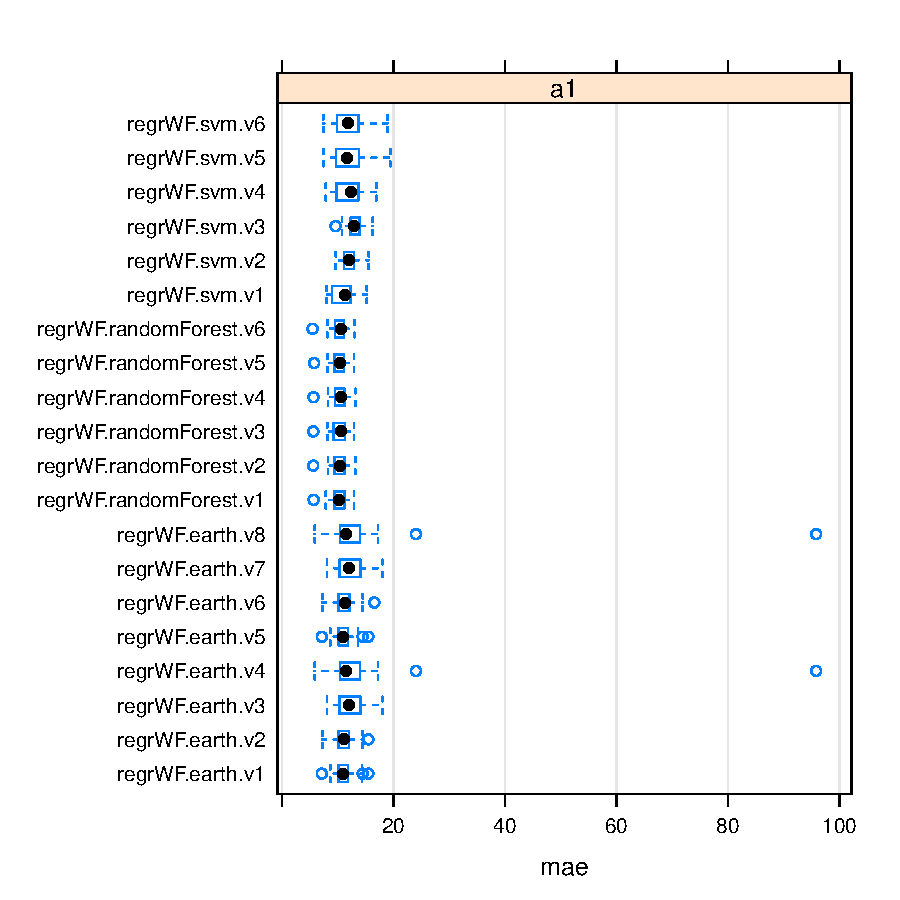
\includegraphics{compExps-030}
  \caption{The MAE results for the task ``a1''.}
  \label{fig:maeA1}
\end{figure}

As before we are using the generic function \texttt{plot()} but this
time applied to a subset of the original object with all results. This
subset is obtained using the generic function \texttt{subset()} that
accepts several parameters to specify the subset we are interested
on. In this case we are using the parameters \texttt{dss} and
\texttt{stats} to indicate that we want to analyze only the results
concerning the task ``a1'' and the metric ``mae''. Other possibilities
are the parameters \texttt{vars} for indicating a subset of the
workflows, and \texttt{its} for indicating a subset of the
iterations. Both \texttt{vars}, \texttt{dss} and \texttt{stats} accept
as values a character string containing a regular expression that will
be used internally with the R function \texttt{grep()} over the vector
of names of the respective objects (names of the workflows, names of
the tasks and names of the metrics, respectively). For instance, if
you want to constrain the previous graph even further to the workflows
whose name ends in ``4'' (absurd example of course!), you could use
the following:

\begin{figure}[ht]
  \centering
\begin{Schunk}
\begin{Sinput}
> plot(subset(res,dss='a1',vars='4$',stats='mae'))
\end{Sinput}
\end{Schunk}
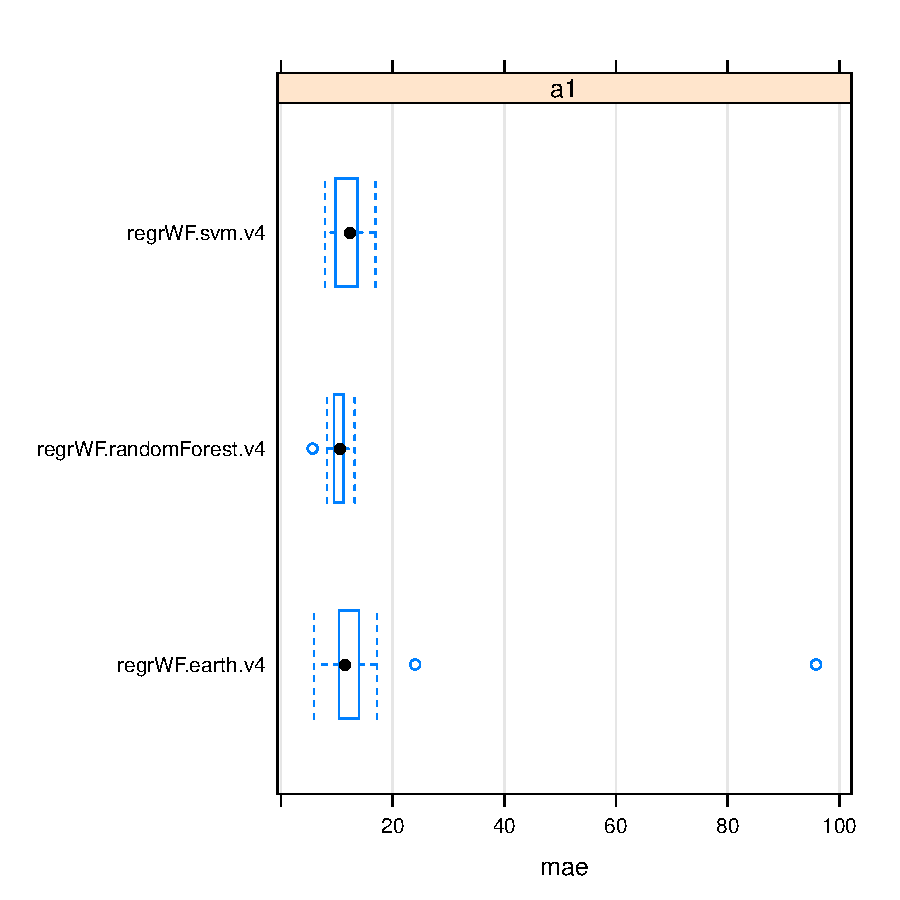
\includegraphics{compExps-031}
  \caption{Illustration of the use of regular expressions in sub-setting the results objects.}
  \label{fig:maeA1b}
\end{figure}
%$

If you are more familiar with the syntax of "wildcards" you may use
the R function \texttt{glob2rx()} to convert to regular expressions,
as show in the following example:

\begin{Schunk}
\begin{Sinput}
> summary(subset(res,dss='a1',vars=glob2rx('*svm*'),stat='mae'))
\end{Sinput}
\begin{Soutput}
== Summary of a  Cross Validation  Experiment ==

 3 x 10 - Fold Cross Validation run with seed =  1234 

* Data sets ::  a1
* Learners  ::  regrWF.svm.v1, regrWF.svm.v2, regrWF.svm.v3, regrWF.svm.v4, regrWF.svm.v5, regrWF.svm.v6

* Summary of Experiment Results:


-> Datataset:  a1 

	*Learner: regrWF.svm.v1 
              mae
avg     11.119022
std      1.948345
min      8.031872
max     15.235946
invalid  0.000000

	*Learner: regrWF.svm.v2 
              mae
avg     12.080142
std      1.353831
min      9.648594
max     15.579599
invalid  0.000000

	*Learner: regrWF.svm.v3 
              mae
avg     13.017781
std      1.435948
min      9.639135
max     16.287188
invalid  0.000000

	*Learner: regrWF.svm.v4 
              mae
avg     12.008268
std      2.413037
min      7.878324
max     16.960718
invalid  0.000000

	*Learner: regrWF.svm.v5 
              mae
avg     11.838932
std      2.796543
min      7.478762
max     19.463476
invalid  0.000000

	*Learner: regrWF.svm.v6 
              mae
avg     11.947164
std      2.814148
min      7.452906
max     18.939631
invalid  0.000000
\end{Soutput}
\end{Schunk}


The following are some illustrations of the use of other available
utility functions.

Obtaining the scores on all iterations and metrics of a workflow on a
particular data set:

\begin{Schunk}
\begin{Sinput}
> getFoldsResults(res,'regrWF.svm.v6','a3')
\end{Sinput}
\begin{Soutput}
        mae        mse
1  3.738376  35.167234
2  5.720053  85.865674
3  3.062192  24.206549
4  4.420911  58.518744
5  6.916167 161.426858
6  3.817921  43.421922
7  5.972168  77.363021
8  2.989061  13.755938
9  3.522196  31.300923
10 4.420862  31.060239
11 7.057749  98.893965
12 3.984418  34.911924
13 3.357721  28.456739
14 4.479078  51.941996
15 5.355505 120.783822
16 3.114532  18.345599
17 5.056947  67.551031
18 4.645389  78.109269
19 3.866368  37.893128
20 3.021332  23.811086
21 2.572863  12.474939
22 3.327102  32.152724
23 2.283692   8.395073
24 5.643101  72.896639
25 3.698872  35.597947
26 5.157141  73.571018
27 5.329479 116.683214
28 4.154213  68.634512
29 4.765092  49.769519
30 4.610539  57.289961
\end{Soutput}
\end{Schunk}

Getting the summary of the results of a particular workflow on a  data set :

\begin{Schunk}
\begin{Sinput}
> getSummaryResults(res,'regrWF.svm.v3','a7')
\end{Sinput}
\begin{Soutput}
             mae        mse
avg     3.060265  28.631648
std     1.062458  25.950318
min     1.462067   4.234327
max     6.195879 110.197624
invalid 0.000000   0.000000
\end{Soutput}
\end{Schunk}

Finally, the \texttt{statScores()} function allows you to apply any
summary function (defaulting to \texttt{mean()}) to the results on a
certain statistic given in parameter \texttt{stat}. The following
calculates the median of the results of the SVMs on the task ``a1'',

\begin{Schunk}
\begin{Sinput}
> statScores(subset(res,vars=glob2rx('*svm*'),dss='a1'),
+            stat='mae',summary='median')
\end{Sinput}
\begin{Soutput}
$a1
regrWF.svm.v1 regrWF.svm.v2 regrWF.svm.v3 regrWF.svm.v4 regrWF.svm.v5 
     11.33815      11.97405      12.98539      12.29963      11.66416 
regrWF.svm.v6 
     11.75567 
\end{Soutput}
\end{Schunk}
%\section{Conclusions}

\bibliographystyle{alpha}
\bibliography{compExps}
\end{document}
